\section{Technický princíp útoku}

\subsection{Základný priebeh web skimmingu}

Útok sa dá rozdeliť na fázy: útočník získa možnosť ovplyvniť obsah stránky alebo niektorý zo skriptov, vloží škodlivý JavaScript (alebo upraví existujúci), kód sa spustí pri otvorení stránky a po vyplnení formulára prečíta a odošle údaje na infraštruktúru útočníka. Krádež sa pritom nemusí odohrať až v databáze: údaje sa kopírujú už počas vypĺňania formulára, takže útok je nebezpečný aj vtedy, keď samotná databáza ani platobná brána neboli prelomené \cite{cisa2020eskimming,pciSsc2025PaymentPage}.

\begin{figure}[H]
    \centering
    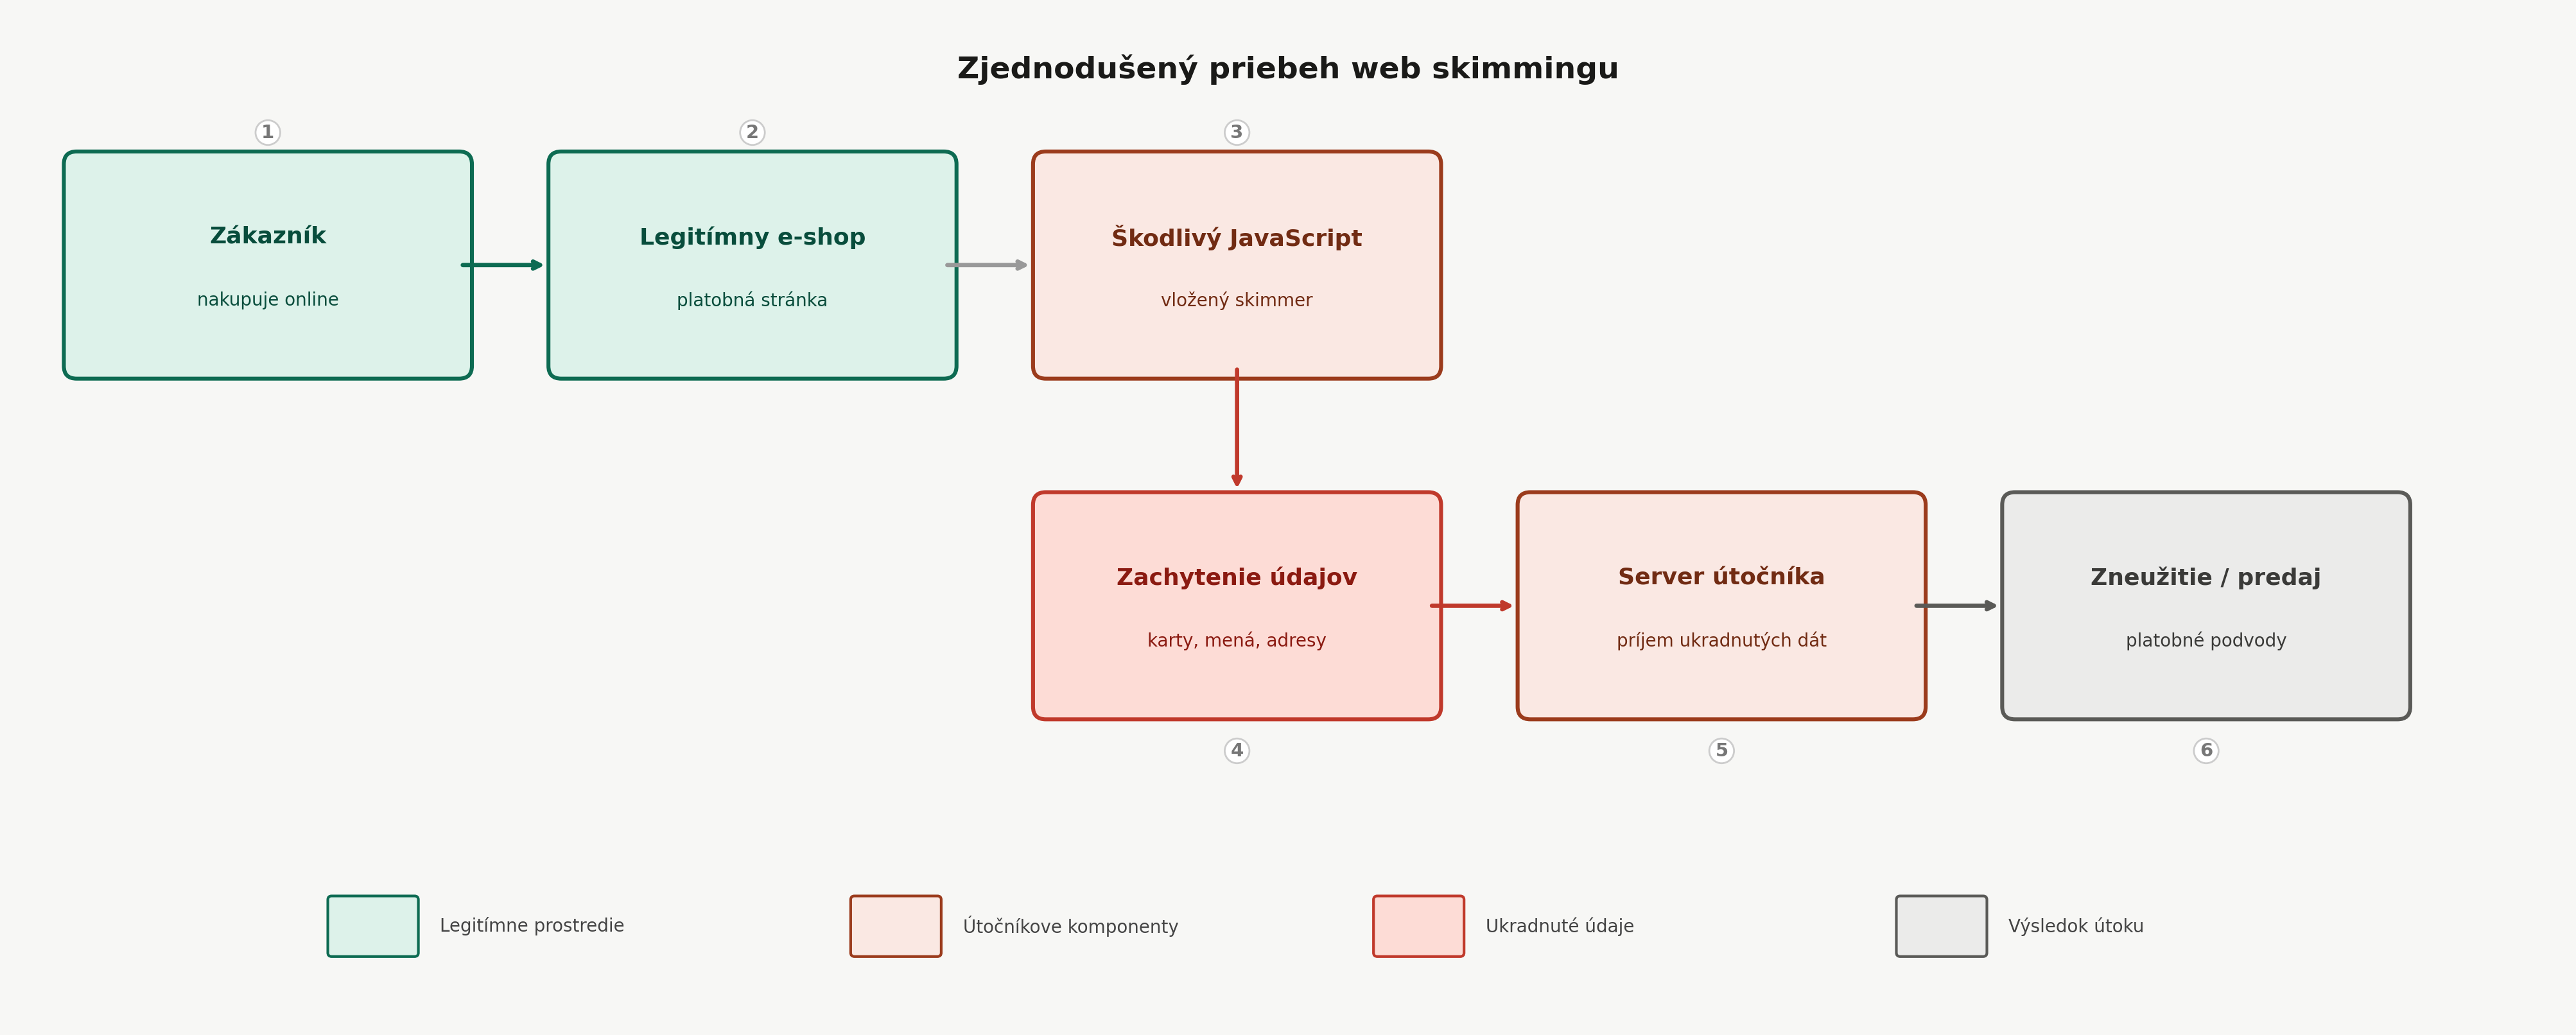
\includegraphics[width=\textwidth]{includes/figures/diagram1_web_skimming_flow.png}
    \caption{Zjednodušený priebeh web skimmingu.}
    \label{fig:web-skimming-flow}
\end{figure}

Web skimming je zároveň útokom na dôveru -- zákazník vidí známu doménu, bežný dizajn a funkčný platobný proces, no na stránke môže paralelne bežať aj kód, ktorý kópiu údajov odošle mimo prostredia obchodníka \cite{pciSsc2025PaymentPage}.

\subsection{Vstupné body a kompromitácia stránky}

Prvou fázou je získanie prístupu k webu alebo k prvku, ktorý sa naň načítava. Útočník nemusí prelomiť hlavný server: stačia slabé prihlasovacie údaje do administrácie, zraniteľný plugin, zastaraná e-commerce platforma, nesprávne nastavené oprávnenia, kompromitovaný účet správcu, prípadne phishing alebo zraniteľný dodávateľ tretej strany \cite{fbi2019eskimming}.

Významným vstupným bodom sú skripty tretích strán -- analytika, reklamné systémy, chatboty, marketingové nástroje, platobné doplnky či knižnice z cudzích serverov. Ak je kompromitovaný takýto externý prvok, útočník nemusí meniť hlavný kód e-shopu; stačí, že sa zmenený skript načíta na stránke zákazníka. OWASP upozorňuje, že jedným z najväčších rizík pri JavaScripte tretích strán je práve kompromitácia servera tretej strany a vloženie škodlivého JavaScriptu do pôvodného skriptu \cite{owaspThirdPartyJavascript,owaspClientSideTop10}.

\begin{figure}[H]
    \centering
    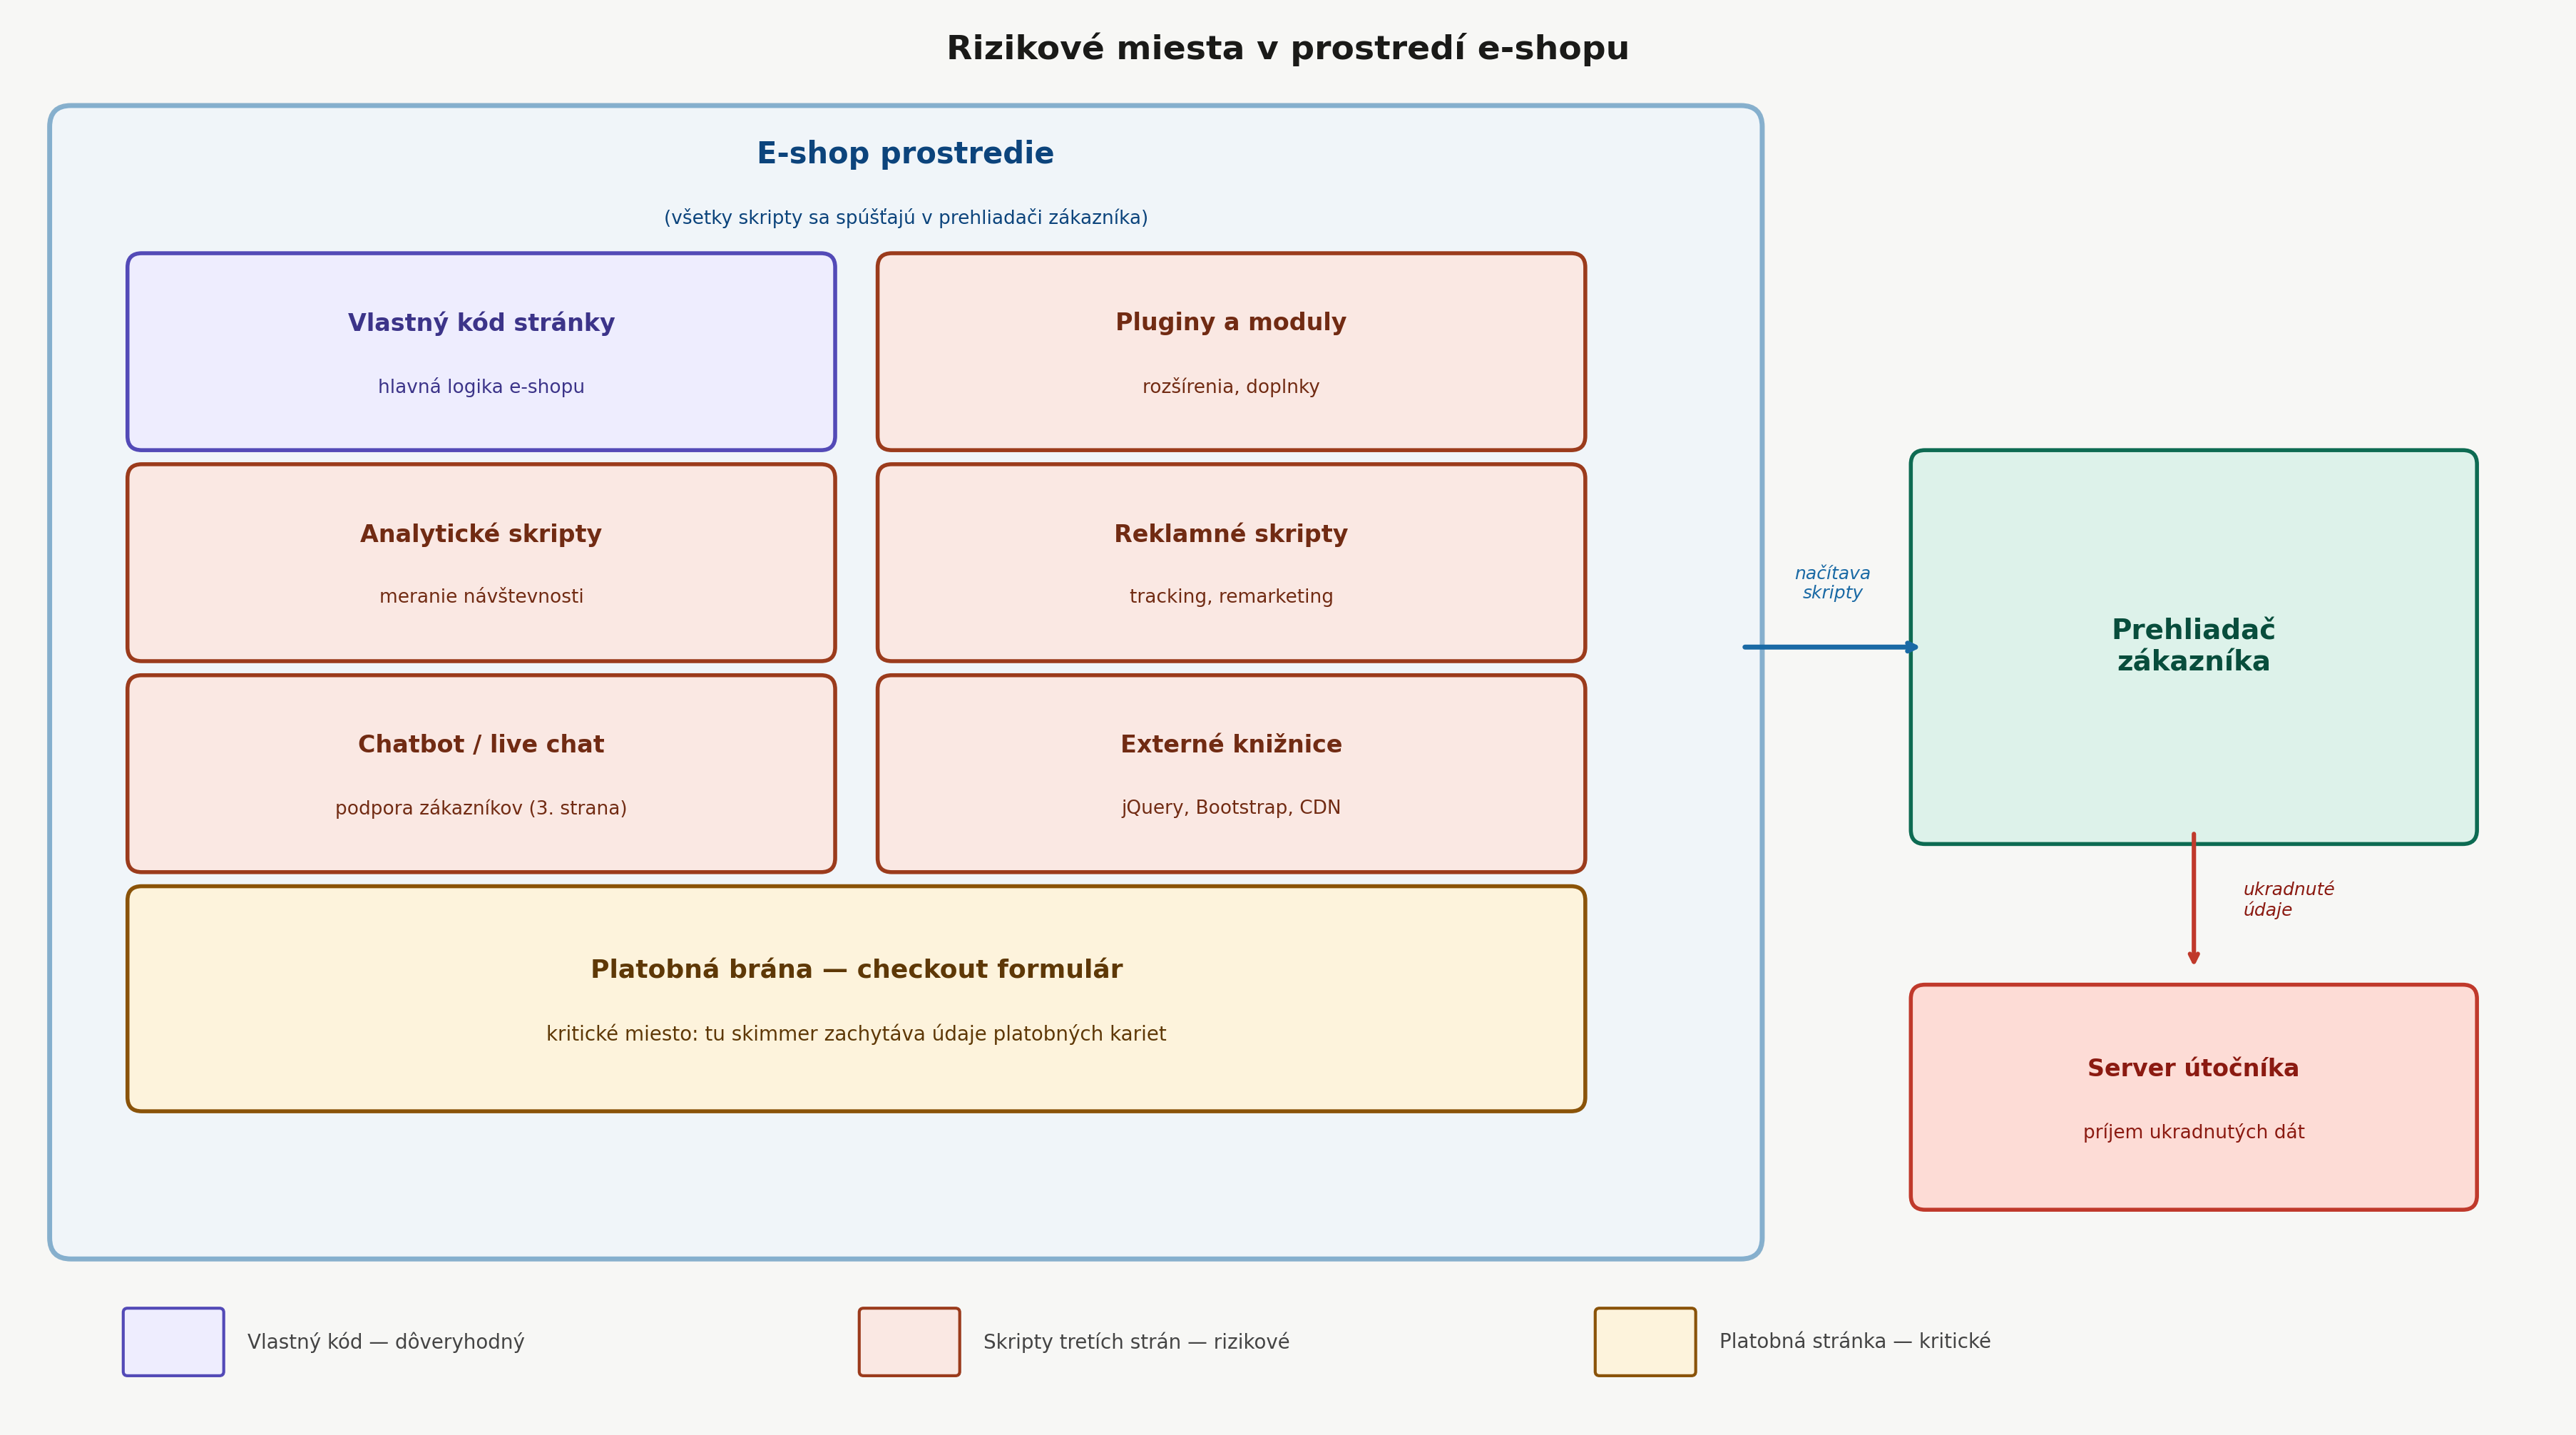
\includegraphics[width=\textwidth]{includes/figures/diagram2_eshop_risk_scripts.png}
    \caption{Rizikové miesta v prostredí e-shopu pri načítavaní klientských skriptov.}
    \label{fig:eshop-risk-scripts}
\end{figure}

Kompromitácia nemusí znamenať prevzatie celého systému -- môže ísť o nenápadnú zmenu v jednom súbore, doplnenie krátkeho skriptu alebo úpravu externého zdroja. Ak útočník navyše obmedzí spustenie kódu iba na stránky s platbou, útok môže byť pre bežného používateľa prakticky neviditeľný.

\subsection{Zachytávanie údajov v prehliadači používateľa}

Po vložení škodlivého JavaScriptu kód pristupuje k hodnotám polí pri vypĺňaní formulára -- meno, priezvisko, e-mail, adresa, telefón, číslo karty, dátum expirácie, bezpečnostný kód. Proces sa odohráva na strane klienta a JavaScript je bežnou súčasťou webov (validácia, interaktivita, výpočty cien, komunikácia s API), takže rovnaké možnosti sa dajú zneužiť na sledovanie polí. Riziko vzniká vtedy, keď sa na citlivej stránke spustí kód, ktorému prevádzkovateľ nerozumie a nedokáže overiť jeho integritu \cite{owaspThirdPartyJavascript,owaspClientSideTop10}.

Útoky sú navyše navrhnuté tak, aby legitímny proces nenarušili: platba prebehne, objednávka sa vytvorí a kópia údajov sa zároveň odošle útočníkovi -- údaje teda môžu byť zachytené ešte pred ich odoslaním platobnej bráne \cite{cisa2020eskimming,pciSsc2025PaymentPage}.

\subsection{Odosielanie údajov a maskovanie útoku}

Po zachytení sa údaje odosielajú na externú infraštruktúru, ktorá nepatrí obchodníkovi ani platobnej bráne. Na stránke s množstvom externých prvkov sa takýto prenos môže stratiť medzi bežnou komunikáciou s analytikou alebo reklamou. Útočníci aktivitu skrývajú: nenápadné názvy súborov, domény pripomínajúce legitímne knižnice, analytické služby alebo CDN, minifikovaný či obfuskovaný JavaScript a spustenie kódu iba na konkrétnych stránkach. Ak správca nekontroluje zoznam načítavaných skriptov a cieľových domén, nemusí si všimnúť, že platobná stránka komunikuje s podozrivým serverom \cite{cisa2020eskimming,pciSsc2025PaymentPage,owaspThirdPartyJavascript,owaspClientSideTop10}.

Jednou z technických obran je Subresource Integrity, ktorá umožňuje prehliadaču overiť, či externý súbor zodpovedá očakávanému hashu, a ak sa zmenil, neprijať ho \cite{owaspSRI}. SRI však nestačí, ak prevádzkovateľ nemá prehľad o skriptoch na platobnej stránke -- preto PCI Security Standards Council zdôrazňuje autorizáciu skriptov, kontrolu integrity a monitorovanie zmien \cite{pciSsc2025PaymentPage}.

\subsection{Prečo je detekcia web skimmingu náročná}

Detekcia je náročná, lebo útok nespôsobuje viditeľnú poruchu webu -- objednávky prechádzajú a obchodník ďalej prijíma platby. Problém sa prejaví až nepriamo: zvýšeným počtom podvodných transakcií, upozornením banky, bezpečnostným skenovaním alebo analýzou sieťovej komunikácie \cite{cisa2020eskimming,pciSsc2025PaymentPage}. Komplikuje to aj dynamická povaha webov a fakt, že útok prebieha na strane klienta -- serverové logy nemusia obsahovať dôkaz o odoslaní údajov tretej strane, lebo to prebieha priamo z prehliadača \cite{owaspClientSideTop10}.

Ochrana preto musí kombinovať serverovú bezpečnosť, kontrolu klientského kódu, monitoring externých zdrojov a pravidelné testovanie platobného procesu. Útočník totiž nemusí prelomiť platobnú bránu ani databázu -- stačí dostať škodlivý JavaScript na miesto, kde používateľ zadáva citlivé údaje \cite{owaspThirdPartyJavascript,pciSsc2025PaymentPage}.
